\chapter{Testing}

This chapter describes the testing of the system, a fundamental part of the development process. It is important to perform testing to ensure that it works as expected. The testing process is divided into two parts: unit testing and system testing. Unit testing is the process of testing individual components of the system while system one is the process of testing the system as a whole.

\section{Automated testing}

% regressions: prevent them while coding
% documentation: enrich the docs of the source functions
% speed: speeds up the development process
% knowledge: you can master the programming language you use

There are several reasons why testing is important. We can group them into four categories:

\begin{itemize}
  \item
        First of all, testing helps to prevent regressions. A regression is a bug that is introduced when a feature is added or especially modified in the system. It helps to prevent them by testing the system after each change. \\
        The unit tests can be defined after the definition of the project, but before writing any code implementation. This way, the developer defines the expected behaviour of the system before writing the code. It is an iterative approach combining programming, unit test creation, and refactoring. This method is called Test-Driven Development (aka TDD), and it is also originated from the Agile manifesto principles~\cite{agile-test-driven-development}. The TDD approach is shown in~\cref{fig:tdd};
  \item
        Documentation: testing helps to enrich the documentation of the source functions. The test cases are a good way to understand the expected behaviour of the system. They can be used as examples to understand how the system works. Compared to separate documentation, the test cases are obviously always updated with the source code, avoiding possible inconsistencies due to the missing update of the documentation after a refactor;
  \item
        The testing process speeds up the development process. It is faster to test the system after each change than to test the system at the end of the development process. It is also easier to find the bugs when they are introduced. The developer can easily identify the cause of the bug and fix it. This way, the developer can focus on the development process rather than the debugging process;
  \item
        Knowledge: testing helps to master the programming language you use. It also helps to understand the best practices of the programming language.
\end{itemize}

\begin{figure}[t]
  \centering
  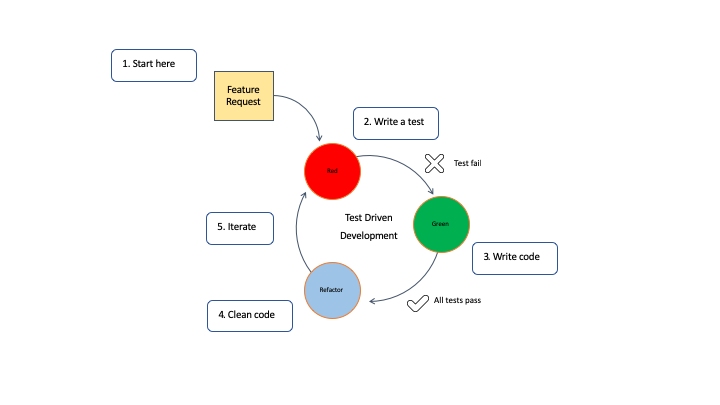
\includegraphics[width=1.0\textwidth]{chapters/06/assets/tdd}
  \caption[Test Driven Development workflow]{Test Driven Development workflow. Image by \texttt{developer.ibm.com}}
  \label{fig:tdd}
\end{figure}

\subsection{Go}

Go is a very versatile programming language. In addition to the description available in~\cref{sec:go-lang} about the characteristics of the language, the testing framework is integrated into the language and provides a simple and efficient way to write tests for functions, methods and interfaces. The testing framework also supports the generation of code coverage reports to identify untested code paths and improve the overall test coverage. Furthermore, it supports the use of table-driven tests, which allow the developer to define test cases in a structured format and iterate over them to execute the tests and also it supports fuzzing, a technique used to discover vulnerabilities in software by providing random or invalid inputs to the program~\cite{go-package-testing}.

Given that the package is a native one, the standard library is enough. Also, it is not included in the compiled binary, enabling the developer to take advantage of the framework without increasing the size of the final binary, where indeed the testing code is not needed at all.

It supports both \textit{Black Box} and \textit{White Box} testing. Black Box testing is a testing technique that focuses on the functionality of the software, used to validate the software against the requirements. White Box, instead, is a testing technique that focuses on the internal structure of the software, used to validate the software against the implementation.

A test file ends with the suffix "\texttt{\_test.go}". The code in the file can be part of the same package of the source file, in order to have visibility on all the private methods and variables, therefore referring to White Box Testing, or in a corresponding package with the \textit{\_test} suffix in order to test the real behaviour, known as Black Box Testing. The test file contains the test functions starting with the prefix "Test" followed by the name of the function to be tested.

To be valid, the testing package must be imported by all the test functions; the main exposed types are:
\begin{itemize}
  \item \texttt{func TestMain(m *testing.M)}: sometimes it is needed to do extra setup before starting the testing; this function is executed before as first. The function takes a pointer to an object which provides methods to control the flow;
  \item \texttt{func TestXxx(t *testing.T)}: the function takes a pointer to an argument providing methods to report the test results;
  \item \texttt{func TestXxx(f *testing.F)}: it is used to perform a fuzz test. If the test fails, we again can use the \texttt{*testing.T} object to report the failure.
  \item \texttt{func BenchmarkXxx(b *testing.B)}: it is used to perform a benchmark test.
\end{itemize}

The Go test runner scans all the test files in the project, runs them based on the given configuration and reports the results to the standard output. The test runner can be configured to run the tests in parallel, in a specific order, or to run only the tests that match a specific pattern. It can also be configured to generate code coverage reports, which can be used to identify untested code paths and improve the overall test coverage.

The \texttt{testing.T} object is used to perform atomic tests, that are the smallest unit of testing. Fuzzing is part of this category and finds out new test cases that might lead to crashes or failures and where the outcomes are not predictable; it is especially useful for strings-based functions and for dealing with user inputs.

\begin{lstlisting}[language=Golang, caption={Go testing framework example file parsing\_test.go}]
package parsing

func TestParseVersionInvalidStringNonNumbers(t *testing.T) {
  _, err := parseVersion("abc")
  if !errors.Is(err, CustomError) {
    t.Errorf("expected CustomError, got %v", err)
  }
}

func TestParseVersionInvalidStringExtraWhitespace(t *testing.T) {
  _, err := parseVersion(" 100")
  if !errors.Is(err, CustomError) {
    t.Errorf("expected CustomError, got %v", err)
  }
}

func TestParseVersionValidStringReturnsCorrectNumber(t *testing.T) {
  result, err := parseVersion("100")
  if err != nil {
    t.Errorf("unexpected error: %v", err)
  }
  expected := 100
  if result != expected {
    t.Errorf("expected %d, got %d", expected, result)
  }
}
\end{lstlisting}

An alternative to the previous syntax is to use the \texttt{t.Run} method and subtests. Doing this way, the syntax would be very similar to how Typescript testing is performed. Anyway, it is not the default convention for the Go coders.

\subsection{Typescript}

Of course, also the cloud app needs to be tested. The chosen testing framework is Jest\footnote{\url{https://jestjs.io}}, part of the OpenJS foundation. Indeed, it is quite similar in terms of concept to the Go testing framework, although it is an external dependency.

A notable syntactical difference is placed in how the files are named and how the evaluation system works; in our configuration, the framework looks for files with the extension ending with \textit{.spec.ts}. Then, all we need is the method named \textit{test} which runs a test. By default, we do not need to define test functions with a uniquely identifiable name, but we \textit{describe} the expected behaviour. For example, the following snippet describes the testing for a utility to parse a valid version number:

\begin{lstlisting}[language=Javascript, caption={Jest testing framework example file parsing.spec.ts}]
[...]
describe('parse version number', () => {
  describe('given an invalid string', () => {
    test('composed of non-numbers throws CustomError', () => {
      expect(() => parseVersion('abc')).toThrow(CustomError);
    });

    test('with extra whitespace throws CustomError', () => {
      expect(() => parseVersion(' 100')).toThrow(CustomError);
    });
  });

  describe('given a valid string', () => {
    it('returns the correct number', () => {
      expect(parseVersion('100')).toBe(100);
    });
  });
});
\end{lstlisting}

The \texttt{expect} function is used to assert the expected behaviour of the system and the \texttt{toThrow} function is used to assert that the function throws an error. The \texttt{toBe} function is used to assert that the function returns the correct value. The \texttt{describe} function is used to group the test cases and the \texttt{test} function is used to define the test cases. The \texttt{it} function is an alias for the \texttt{test} function.

\subsection{Snyk}

We also use Snyk to scan for vulnerabilities in the dependencies of the tool project. Snyk offers a CLI tool embedded in a container image\footnote{\url{https://hub.docker.com/r/snyk/snyk}}. We run the \texttt{golang-1.22} tagged version to get the results. The tool is very useful to find out the vulnerabilities in the dependencies and to fix them. In our case, we found a vulnerability in a package, that we fixed by updating the package to the latest available version.

This software is also specialized in finding vulnerabilities in NodeJS projects; therefore, we use it to scan the cloud web app project, in addition to the \textit{audit} command provided by the NodeJS package manager \texttt{npm}. The tagged version we use is \texttt{node-22}. Due to the way the dependencies proliferate and the number of discovered vulnerabilities each day, it is important to run the tool frequently to keep the project secure.

An example of commands to issue for scanning dependencies in a Go project is the following:
\begin{mdframed}
  \texttt{\$ export SNYK\_TOKEN=token}\\
  \texttt{\$ docker run --rm -it --env SNYK\_TOKEN -v \$(pwd):/app snyk/snyk:golang-1.22}
\end{mdframed}
The \texttt{SNYK\_TOKEN} is an environment variable that contains the token to authenticate the user to the Snyk service. The \texttt{-v} flag is used to mount the current directory to the \texttt{/app} directory in the container. The \texttt{--rm} flag is used to remove the container at the end and the \texttt{-it} flag is used to run the container in interactive mode to see the output of the command.

\section{Manual system testing}

In addition to the automated testing, the functionalities of the products are tested by a real group of people. In fact, the company has a dedicated testing team composed by six people, located in the Indian offices. They take care of the manual testing of the system. To synchronize the work, we do a weekly stand-up meeting focused on the completed tests and on the upcoming ones. The team is divided into different groups: there is the group in charge of testing the infrastructure, the group in charge of testing the frontend, and the group in charge of testing the backend.

Once the implementation of the stories related to a functionality is completed, they are taken in charge by this team which performs several tests, with and without reading the documentation: the latter to test the usability of the system as the final customer and the former with the goal to test the expected behaviour in a real environment.

If the manual test does not pass the minimum requirements, the ticket related to that story is reopened and therefore handled by the developer again. After that the fixes are applied, the ticket is assigned back to the testers, and so on. If the testers are satisfied with the implementation, the ticket is closed and the story is considered done, and the feature is ready to be released.

\section{Considerations}

We wrote more than two hundred test cases, including various parameter combinations and edge cases. We used the two syntaxes described in the previous subsections respectively for the two programming languages and we also took advantage of the table-driven tests to test the same function with different parameters.

Despite the automated testing, sometimes the testers still report troubles with test cases not handled by the developer. This is another good way to improve the test coverage.

In our personal projects, we never had a so defined and strict testing methodology. TDD is really such a new concept for us, but it is essential to be efficient in the development process because it helps to focus on the actual requirements of the system. It is also a good way to understand the expected behaviour of the system and to identify the edge cases that need to be handled.
